Similarly, the unique edge in the TN representing the trace of a matrix corresponds to expressing the TN~(which is a scalar) as a sum of scalars~(the diagonal entries of the matrix), let $\Ab\in\RR^{d\times d}$:
$$\begin{tikzpicture}[baseline=\baseline]
    \tikzset{tensor/.style = {minimum size = 0.5cm,shape = circle,thick,draw=black,inner sep = 0pt}, edge/.style = {thick,line width=.4mm},every loop/.style={}}
    \def\y{0}
    \def\x{0}
    \node[tensor,fill=red!50!white] (A) at (\x,\y+0.2){\scalebox{0.85}{$\Ab$}};
    \draw[edge] (A) to [out=-20,in=-160, distance=1.35cm] (A);
    \draw[dotted] (\x-0.15,\y-0.1) -- (\x-0.15,\y-0.8);
    \node[draw=none] () at (\x,\y-0.4) {\scalebox{0.7}{\dimcolor{$d$}}};
\end{tikzpicture}\hspace{-0.7cm}
=
\sum_{i=1}^d\left(
\begin{tikzpicture}[baseline=\baseline]
    \tikzset{tensor/.style = {minimum size = 0.5cm,shape = circle,thick,draw=black,inner sep = 0pt}, edge/.style = {thick,line width=.4mm},every loop/.style={}}
    \def\y{0}
    \def\x{0}
    \node[tensor,fill=red!50!white] (A) at (\x,\y){\scalebox{0.85}{$\Ab$}};
     \draw[edge] (\x-0.25,\y) to [out=110,in=60, distance=0.1cm] (\x-0.6,\y-0.2);    
    \draw[edge] (\x+0.25,\y) to [out=110,in=60, distance=0.1cm] (\x+0.6,\y-0.2); 
    \node[draw=none] () at (\x+0.7,\y-0.25) {\scalebox{0.7}{\indcolor{$i$}}};
    \node[draw=none] () at (\x-0.7,\y-0.25) {\scalebox{0.7}{\indcolor{$i$}}};
    \end{tikzpicture}\right)=\sum_{i=1}^d\Ab_{ii}.
    $$
Consider now a more interesting example:
$$\begin{tikzpicture}[baseline=\baseline]
    \tikzset{tensor/.style = {minimum size = 0.5cm,shape = circle,thick,draw=black,inner sep = 0pt}, edge/.style = {thick,line width=.4mm},every loop/.style={}}
    \def\y{0}
    \def\x{0}
    \node[tensor,fill=red!50!white] (A) at (\x,\y+0.5){\scalebox{0.85}{$\Ab$}};
    \node[tensor,fill=red!50!white] (B) at (\x,\y-0.5){\scalebox{0.85}{$\Bb$}};
    \draw[edge](A)--(B)node [midway, right] {\scalebox{0.7}{\dimcolor{$R$}}};
    \draw[edge](A) -- (\x+0.5,\y+0.5)--(\x+0.5,\y)--(\x+1,\y)node [midway, above] {\scalebox{0.7}{\dimcolor{$n$}}};
    \draw[edge](A) -- (\x-0.5,\y+0.5)--(\x-0.5,\y)--(\x-1,\y)node [midway, above] {\scalebox{0.7}{\dimcolor{$m$}}};
    \draw[edge](B) -- (\x+0.5,\y-0.5)--(\x+0.5,\y-0.1)--(\x+1,\y-0.1)node [midway, below] {\scalebox{0.7}{\dimcolor{$q$}}};
    \draw[edge](B) -- (\x-0.5,\y-0.5)--(\x-0.5,\y-0.1)--(\x-1,\y-0.1)node [midway, below] {\scalebox{0.7}{\dimcolor{$p$}}};
    \end{tikzpicture}.$$
The edge in this TN corresponds to a way to express the matrix represented by the TN as a sum of matrices:
$$\begin{tikzpicture}[baseline=\baseline]
    \tikzset{tensor/.style = {minimum size = 0.5cm,shape = circle,thick,draw=black,inner sep = 0pt}, edge/.style = {thick,line width=.4mm},every loop/.style={}}
    \def\y{0}
    \def\x{0}
    \node[tensor,fill=red!50!white] (A) at (\x,\y+0.5){\scalebox{0.85}{$\Ab$}};
    \node[tensor,fill=red!50!white] (B) at (\x,\y-0.5){\scalebox{0.85}{$\Bb$}};
    \draw[edge](A)--(B)node [midway, right] {\scalebox{0.7}{\dimcolor{$R$}}};
    \draw[edge](A) -- (\x+0.5,\y+0.5)--(\x+0.5,\y)--(\x+1,\y)node [midway, above] {\scalebox{0.7}{\dimcolor{$n$}}};
    \draw[edge](A) -- (\x-0.5,\y+0.5)--(\x-0.5,\y)--(\x-1,\y)node [midway, above] {\scalebox{0.7}{\dimcolor{$m$}}};
    \draw[edge](B) -- (\x+0.5,\y-0.5)--(\x+0.5,\y-0.1)--(\x+1,\y-0.1)node [midway, below] {\scalebox{0.7}{\dimcolor{$q$}}};
    \draw[edge](B) -- (\x-0.5,\y-0.5)--(\x-0.5,\y-0.1)--(\x-1,\y-0.1)node [midway, below] {\scalebox{0.7}{\dimcolor{$p$}}};
    \draw[dotted](\x+0.35,\y+0.15) -- (\x-0.35,\y+0.15);
    \end{tikzpicture}
    =
    \sum_{r=1}^R\begin{tikzpicture}[baseline=\baseline]
    \tikzset{tensor/.style = {minimum size = 0.5cm,shape = circle,thick,draw=black,inner sep = 0pt}, edge/.style = {thick,line width=.4mm},every loop/.style={}}
    \def\y{0}
    \def\x{0}
    \node[tensor,fill=red!50!white] (A) at (\x,\y+1){\scalebox{0.85}{$\Ab$}};
    \node[tensor,fill=red!50!white] (B) at (\x,\y-1){\scalebox{0.85}{$\Bb$}};
    \draw[edge](A) -- (\x,\y+0.45)node [pos=1.4]{\scalebox{0.7}{\indcolor{$r$}}};
    \draw[edge](B) -- (\x,\y-0.45)node [pos=1.3]{\scalebox{0.7}{\indcolor{$r$}}};
    \draw[edge](A) -- (\x+0.5,\y+1)--(\x+0.5,\y)--(\x+1,\y)node [midway, above] {\scalebox{0.7}{\dimcolor{$n$}}};
    \draw[edge](A) -- (\x-0.5,\y+1)--(\x-0.5,\y)--(\x-1,\y)node [midway, above] {\scalebox{0.7}{\dimcolor{$m$}}};
    \draw[edge](B) -- (\x+0.5,\y-1)--(\x+0.5,\y-0.1)--(\x+1,\y-0.1)node [midway, below] {\scalebox{0.7}{\dimcolor{$q$}}};
    \draw[edge](B) -- (\x-0.5,\y-1)--(\x-0.5,\y-0.1)--(\x-1,\y-0.1)node [midway, below] {\scalebox{0.7}{\dimcolor{$p$}}};
    \end{tikzpicture}
    =
    \sum_{r=1}^R\Ab_r\kron\Bb_r.$$
We recognize here that this TN corresponds to a sum of Kronecker products! 
\paragraph{Tensors, Multilinear Maps and Polynomials.}
We can think of tensors as \emph{representations of multi-linear maps}, in exactly the same sense that matrices represent linear maps. Recall that a matrix $\Ab\in\RR^{m\times n}$ represents a linear map $\RR^n\to\RR^m$ via $\xb\mapsto \Ab\xb$. In tensor network notation, this is simply
$$
\yb = \Ab\xb
=
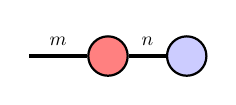
\begin{tikzpicture}[baseline=-0.5ex]
    \tikzset{tensor/.style = {minimum size = 0.5cm,shape = circle,thick,draw=black,inner sep = 0pt},
             edge/.style   = {thick,line width=.4mm},every loop/.style={}}
    \def\x{0}\def\y{0}
    \node[tensor,fill=red!50!white] (A) at (\x,\y){$\Ab$};
    \node[tensor,fill=blue!20!white] (x) at (\x+1,\y){$\xb$};
    \draw[edge] (A) -- (x) node [midway,above]{\scalebox{0.7}{\dimcolor{$n$}}};
    \draw[edge] (A) -- (\x-1,\y) node [midway,above]{\scalebox{0.7}{\dimcolor{$m$}}};
\end{tikzpicture}
\in\RR^{m}.
$$
Linearity means that $\Ab(\alpha \xb+\beta \zb)=\alpha \Ab\xb+\beta \Ab\zb$ for all $\alpha,\beta\in\RR$ and $\xb,\zb\in\RR^n$. A tensor is the natural generalization when the map is linear \emph{in several arguments separately}. Concretely, an order-$N$ tensor $\Tt\in\RR^{d_1\times\cdots\times d_N}$ defines a map that takes $N$ input vectors and returns a scalar by contracting along all modes:
$$
f(\xb^{(1)},\dots,\xb^{(N)})
:= \langle \Tt,\ \xb^{(1)}\outprod \cdots \outprod \xb^{(N)}\rangle
=
\sum_{i_1=1}^{d_1}\cdots\sum_{i_N=1}^{d_N}\Tt_{i_1\cdots i_N}\,\xb^{(1)}_{i_1}\cdots \xb^{(N)}_{i_N}.
$$
This map is \emph{multi-linear}: it is linear in each $\xb^{(k)}$ when the other vectors are fixed. In tensor network diagrams, this is simply
\[
f(\ab,\bb,\dots,\zb)
=
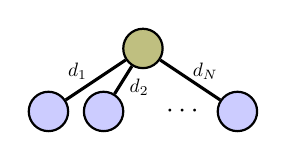
\begin{tikzpicture}[baseline=2ex]
    \tikzset{tensor/.style = {minimum size = 0.5cm,shape = circle,thick,draw=black,inner sep = 0pt},
             edge/.style   = {thick,line width=.4mm},
             every loop/.style={}}
    \def\x{0}\def\y{0}

    \node[tensor,fill=green!50!red!50!white] (T) at (\x,\y+0.8){$\Tt$};

    \node[tensor,fill=blue!20!white] (a) at (\x-1.2,\y){$\ab$};
    \node[tensor,fill=blue!20!white] (b) at (\x-0.5,\y){$\bb$};
    \node[draw=none] (dots) at (\x+0.5,\y){$\cdots$};
    \node[tensor,fill=blue!20!white] (z) at (\x+1.2,\y){$\zb$};

    \draw[edge] (T) -- (a) node [near end,above]{\scalebox{0.7}{\dimcolor{$d_1\ $}}};
    \draw[edge] (T) -- (b) node [near end,right]{\scalebox{0.7}{\dimcolor{$d_2$}}};
    \draw[edge] (T) -- (z) node [near end,above]{\scalebox{0.7}{\dimcolor{$d_N$}}};
\end{tikzpicture}
\in\RR,
\]
where $\ab, \bb,\cdots,\zb\in\RR^d$.
If we leave one leg open, we obtain a \emph{vector-valued} multi-linear map. For instance, if $\Tt\in\RR^{d_1\times\cdots\times d_N \times p}$, contracting all modes except the last defines a multi-linear map whose output is a vector of dimension $p$:
$$
f(\ab,\bb,\dots,\zb)
=
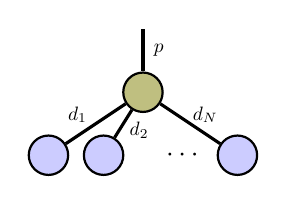
\begin{tikzpicture}[baseline=2ex]
    \tikzset{tensor/.style = {minimum size = 0.5cm,shape = circle,thick,draw=black,inner sep = 0pt},
             edge/.style   = {thick,line width=.4mm},
             every loop/.style={}}
    \def\x{0}\def\y{0}

    \node[tensor,fill=green!50!red!50!white] (T) at (\x,\y+0.8){$\Tt$};

    \node[tensor,fill=blue!20!white] (a) at (\x-1.2,\y){$\ab$};
    \node[tensor,fill=blue!20!white] (b) at (\x-0.5,\y){$\bb$};
    \node[draw=none] (dots) at (\x+0.5,\y){$\cdots$};
    \node[tensor,fill=blue!20!white] (z) at (\x+1.2,\y){$\zb$};

    \draw[edge] (T) -- (a) node [near end,above]{\scalebox{0.7}{\dimcolor{$d_1\ $}}};
    \draw[edge] (T) -- (b) node [near end,right]{\scalebox{0.7}{\dimcolor{$d_2$}}};
    \draw[edge] (T) -- (z) node [near end,above]{\scalebox{0.7}{\dimcolor{$d_N$}}};
    \draw[edge] (T) -- (\x,\y+1.6) node [midway,right]{\scalebox{0.7}{\dimcolor{$p$}}};
\end{tikzpicture}
\in\RR^p.
$$

